\documentclass[12pt,a4paper,oldfontcommands]{memoir}
\usepackage[utf8]{inputenc}
\usepackage[T1]{fontenc}
\usepackage{microtype}
\usepackage[dvips]{graphicx}
\usepackage{subcaption}
\setlength{\parindent}{1em}
\setlength{\parskip}{0.8em}

\usepackage[
    breaklinks=true,colorlinks=true,
%linkcolor=blue,urlcolor=blue,citecolor=blue,% PDF VIEW
    linkcolor=black,urlcolor=black,citecolor=black,% PRINT
    bookmarks=true,bookmarksopenlevel=2]{hyperref}

\usepackage{geometry}
% PDF VIEW
% \geometry{total={210mm,297mm},
% left=25mm,right=25mm,%
% bindingoffset=0mm, top=25mm,bottom=25mm}
% PRINT
\geometry{total={210mm,297mm},
    left=20mm,right=20mm,
    bindingoffset=10mm, top=25mm,bottom=25mm}

\OnehalfSpacing

%%% CHAPTER'S STYLE
\chapterstyle{bianchi}
%\chapterstyle{ger}
%\chapterstyle{madsen}
%\chapterstyle{ell}
%%% STYLE OF SECTIONS, SUBSECTIONS, AND SUBSUBSECTIONS
\setsecheadstyle{\Large\bfseries\sffamily\raggedright}
\setsubsecheadstyle{\large\bfseries\sffamily\raggedright}
\setsubsubsecheadstyle{\bfseries\sffamily\raggedright}


%%% STYLE OF PAGES NUMBERING
%\pagestyle{companion}\nouppercaseheads
%\pagestyle{headings}
%\pagestyle{Ruled}
\pagestyle{plain}
\makepagestyle{plain}
\makeevenfoot{plain}{\thepage}{}{}
\makeoddfoot{plain}{}{}{\thepage}
\makeevenhead{plain}{}{}{}
\makeoddhead{plain}{}{}{}


\maxsecnumdepth{subsection} % chapters, sections, and subsections are numbered
\maxtocdepth{subsection} % chapters, sections, and subsections are in the Table of Contents






%MOJE USTAWIENIA-------------------------------------------------------------------------

\usepackage[polish]{babel}
\usepackage{listings}
\renewcommand{\lstlistingname}{Kod}
\usepackage{color}
\usepackage[colorinlistoftodos]{todonotes}
\usepackage{amsthm}
\usepackage{longtable}
\usepackage{pdflscape}
\usepackage{graphicx}
\usepackage{color, colortbl}
\usepackage{pgfplots}
\usepackage{subcaption}
\usepackage{url}
\usepackage[resetlabels,labeled]{multibib}
\usepackage{framed}
\usepackage{lipsum}
\usepackage{amsmath}

\usepackage{amsthm}
\usepackage{enumerate}
\usepackage{mathrsfs}
\usepackage[normalem]{ulem}
\usepackage{float}
\usepackage{multicol}

\usepackage{caption}


\captionsetup[table]{name=Tabela}

\theoremstyle{plain}
\newtheorem{theorem}{Theorem}[chapter]
\newtheorem{prop}[theorem]{Proposition}
\newtheorem{corollary}[theorem]{Corollary}
\newtheorem{lemma}[theorem]{Lemma}


\theoremstyle{definition}
\newtheorem{defn}[theorem]{Definicja}
\newtheorem{ex}[theorem]{Przykład}
\newtheorem{exer}[theorem]{Ćwiczenie}
\newtheorem{refer}[theorem]{Reflection}

\theoremstyle{remark}
\newtheorem{remark}[theorem]{Remark}
\newtheorem{note}[theorem]{Note}
\newtheorem{caut}[theorem]{CAUTION}

% set the default code style
\lstset{
    frame=tb, % draw a frame at the top and bottom of the code block
    tabsize=4, % tab space width
    showstringspaces=false, % don't mark spaces in strings
    numbers=left, % display line numbers on the left
    commentstyle=\color{green}, % comment color
    keywordstyle=\color{blue}, % keyword color
    stringstyle=\color{darkred} % string color
}



\definecolor{dkgreen}{rgb}{0,0.6,0}
\definecolor{gray}{HTML}{d9d9d9}
\definecolor{mauve}{HTML}{ffe6e6}

\newcites{New}{The other list}
\lstset{frame=tb,
    language=Java,
    aboveskip=3mm,
    belowskip=3mm,
    showstringspaces=false,
    columns=flexible,
    basicstyle={\small\ttfamily},
    numbers=none,
    numberstyle=\tiny\color{gray},
    keywordstyle=\color{blue},
    commentstyle=\color{dkgreen},
    stringstyle=\color{red},
    breaklines=true,
    breakatwhitespace=true,
    tabsize=3,
}
% for placeholder text
\usepackage{lipsum}


\newtheorem{mydef}{Definition}


\renewcommand\appendixtocname{Dodatki}
\renewcommand\appendixpagename{Dodatki}

\renewcommand\lstlistingname{Pseudokod}
\renewcommand\lstlistlistingname{Spis pseudokodów}

\newcommand{\AR}[1]{\todo[inline, color=blue!30]{AR: #1}}
\newcommand{\MM}[1]{\todo[inline, color=green!30]{MM: #1}}

\newcommand{\HRule}{\rule{\linewidth}{0.5mm}} % Defines a new command for the horizontal lines, change thickness here



% \usepackage[T1]{fontenc}
% \usepackage[utf8]{inputenc}
% \usepackage{indentfirst}
% \usepackage{icomma}
% \usepackage{xcolor}
% \usepackage{graphicx}
% \usepackage{float}
% \usepackage{longtable}
% \usepackage{url}
% \urlstyle{same}
% \brokenpenalty=1000
% \clubpenalty=1000
% \widowpenalty=1000
% % \renewcommand\refname{Bibliografia}
% \renewcommand{\contentsname}{Spis Treści}
% \renewcommand{\listfigurename}{Spis Rycin}
% \renewcommand{\listtablename}{Spis Tabel}
% \renewcommand{\figurename}{Rycina}
% \renewcommand{\tablename}{Tabela}
% \chapterstyle{bianchi}
% \usepackage{etoolbox}
% \usepackage[utf8]{inputenx}
% \usepackage{indentfirst}
% \usepackage{microtype}
% \usepackage{lettrine}
% \usepackage{diagbox}
% \usepackage{titlesec}
% \usepackage[nottoc, notlof, notlot]{tocbibind}
% \usepackage{caption}
% \patchcmd{\thebibliography}{\section*}{\section}{}{}
%     \usepackage{xcolor}
%     \usepackage{lipsum} % dummy text for the MWE


% % Put % before of what you want disabled

% % Select what to do with todonotes:
% % \usepackage[disable]{todonotes} % notes not showed
% \usepackage[draft]{todonotes}   % notes showed

% % Select what to do with command \comment:
% % \newcommand{\comment}[1]{}  %comment not showed
% \newcommand{\comment}[1]
% {\par {\bfseries \color{blue} #1 \par}} %comment showed


\begin{document}
    \begin{figure}
        \centerline{
\includegraphics{uj.jpg}}
        \label{fig}
    \end{figure}
    \begin{center}
        \large
        Uniwersytet Jagielloński\\
        Wydział Matematyki i Informatyki\\
        \Large
        Instytut Informatyki i Matematyki
        Komputerowej\\
        \smallskip
        \large
        Studia dzienne
    \end{center}
    \smallskip
    \begin{center}
        \large
        Miraslau Douher
    \end{center}

    \smallskip
    \begin{center}
        \Large
        \begin{center}
            \large
            Praca magisterska
        \end{center}
        \Large
        \textbf{Analiza efektywności generowania Operatorów mutacyjnych (Mutantów) poprzez duże modele językowe}
    \end{center}

    \vfill
    \begin{center}
        \large
        Opiekunowie: \\

    \end{center}

    \medskip
    \begin{center}
        dr. prof. Michał Mnich

        \Large
        \medskip
        Kraków 2026
    \end{center}


    \normalsize
    \clearpage
    \tableofcontents

    \newpage
    \listoffigures

    \newpage
    \listoftables

    \newpage
    \lstlistoflistings

    \newpage

    \begin{abstract}
        Lorem ipsum dolor sit amet, consectetur adipiscing elit, sed do eiusmod tempor incididunt ut labore et dolore magna aliqua. Ut enim ad minim veniam, quis nostrud exercitation ullamco laboris nisi ut aliquip ex ea commodo consequat. Duis aute irure dolor in reprehenderit in voluptate velit esse cillum dolore eu fugiat nulla pariatur. Excepteur sint occaecat cupidatat non proident, sunt in culpa qui officia deserunt mollit anim id est laborum..


    \end{abstract}

    \cleardoublepage

    \chapter{Wstęp}
    \section{Section01}

    Lorem ipsum dolor sit amet, consectetur adipiscing elit, sed do eiusmod tempor incididunt ut labore et dolore magna aliqua. Ut enim ad minim veniam, quis nostrud exercitation ullamco laboris nisi ut aliquip ex ea commodo consequat. Duis aute irure dolor in reprehenderit in voluptate velit esse cillum dolore eu fugiat nulla pariatur. Excepteur sint occaecat cupidatat non proident, sunt in culpa qui officia deserunt mollit anim id est laborum.
    \cite{cyt01}.

    \newpage
    \section{Section01y}
    Lorem ipsum dolor sit amet, consectetur adipiscing elit, sed do eiusmod tempor incididunt ut labore et dolore magna aliqua. Ut enim ad minim veniam, quis nostrud exercitation ullamco laboris nisi ut aliquip ex ea commodo consequat. Duis aute irure dolor in reprehenderit in voluptate velit esse cillum dolore eu fugiat nulla pariatur. Excepteur sint occaecat cupidatat non proident, sunt in culpa qui officia deserunt mollit anim id est laborum.

    \begin{itemize}
        \item Lorem ipsum dolor sit amet, consectetur adipiscing elit, sed do eiusmod tempor incididunt ut labore et dolore magna aliqua. Ut enim ad minim veniam, quis nostrud exercitation ullamco laboris nisi ut aliquip .
        \item Lorem ipsum dolor sit amet, consectetur adipiscing elit, sed do eiusmod tempor incididunt ut labore et dolore magna aliqua. Ut enim ad minim veniam, quis nostrud exercitation ullamco laboris nisi ut aliquip ex ea commodo consequat. Duis aute irure dolor in reprehenderit in voluptate velit esse.
    \end{itemize}


    \begin{figure}[ht]
        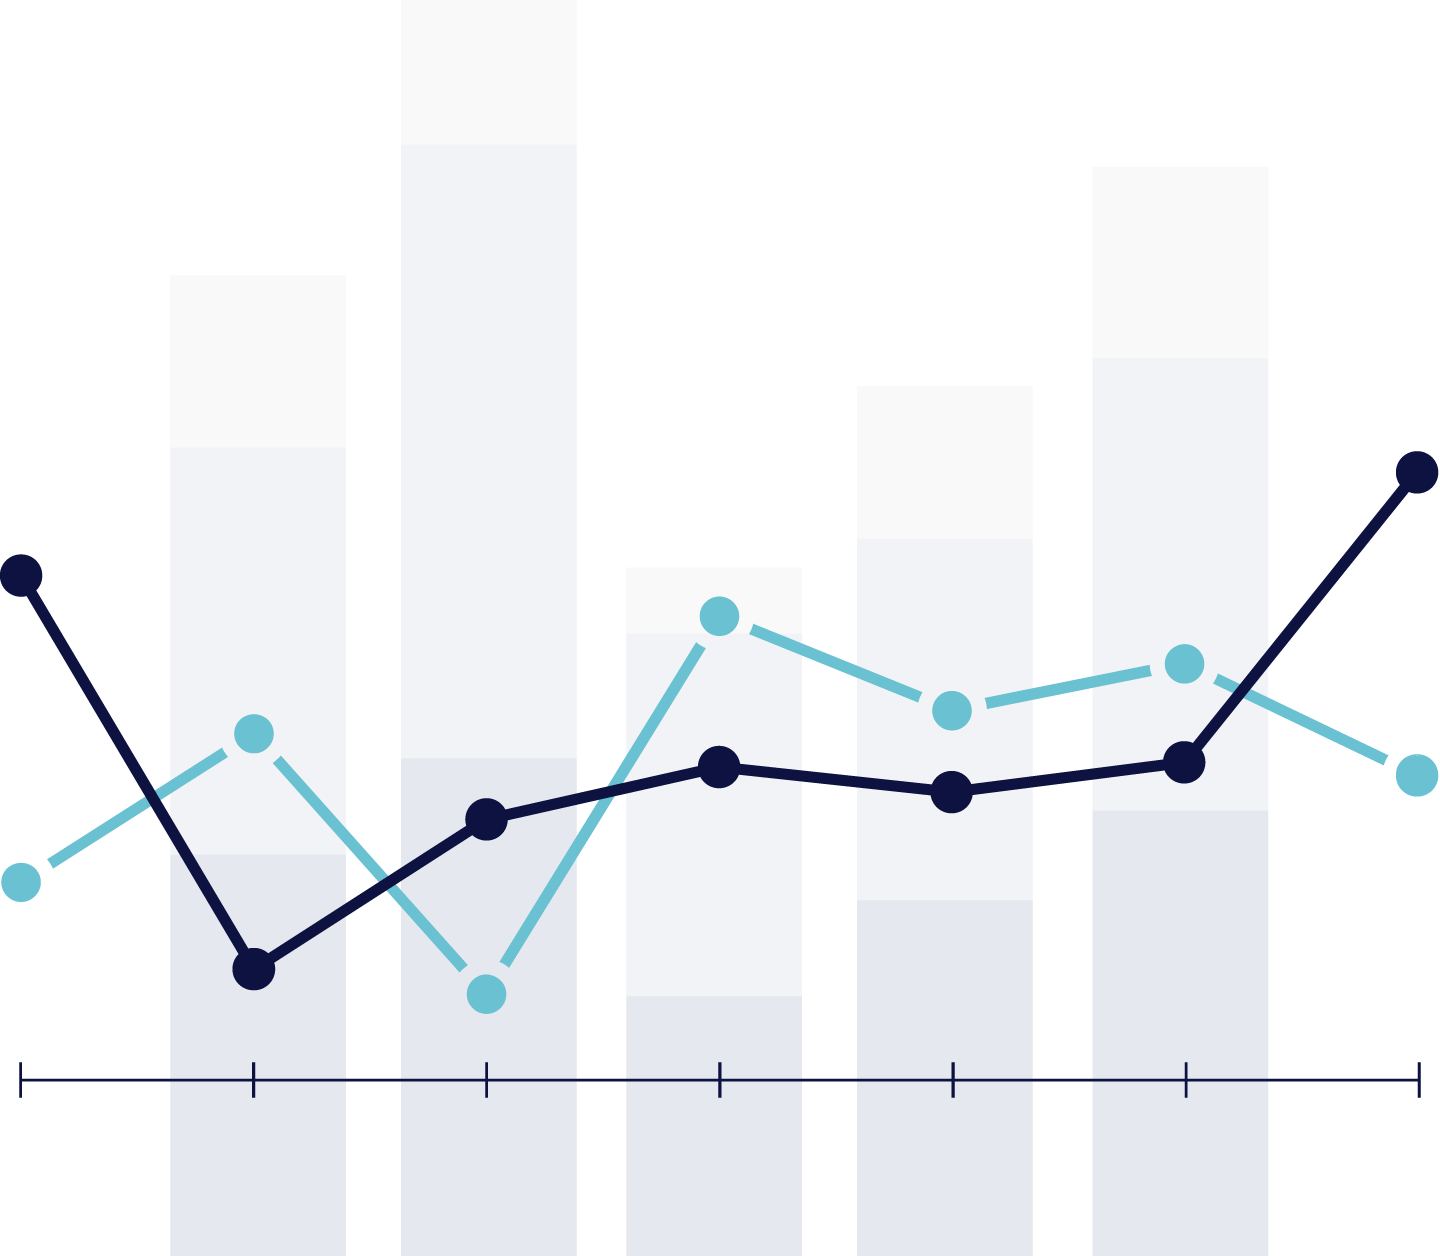
\includegraphics[width=1\textwidth]{pic01.png}
        \caption{Lorem ipsum dolor sit amet, consectetur adipiscing elit}
        \label{fig:proces}
    \end{figure}


    \section{Section03}

    Lorem ipsum dolor sit amet, consectetur adipiscing elit, sed do eiusmod tempor incididunt ut labore et dolore magna aliqua. Ut enim ad minim veniam, quis nostrud exercitation ullamco laboris nisi ut aliquip .

    \subsection{SubSection01}
    Lorem ipsum dolor sit amet, consectetur adipiscing elit, sed do eiusmod tempor incididunt ut labore et dolore magna aliqua. Ut enim ad minim veniam, quis nostrud exercitation ullamco laboris nisi ut aliquip .


    \begin{lstlisting}[language=C++, caption={Lorem ipsum dolor}]
3 * 2;
x = 3 * e;
x = 3 * 42;
    \end{lstlisting}



    \begin{table}[H]
        \centering
        \begin{tabular}{|l|c|c|}
            \hline
            & Moduł Alfa & Moduł Beta \\ \hline
            \footnotesize{Parametr pierwszy} & 12 & 19 \\ \hline
            \footnotesize{Parametr drugi} & 4 & 7 \\ \hline
            \footnotesize{Parametr trzeci} & 23 & 15 \\ \hline
            \footnotesize{Parametr czwarty} & 154 & 203 \\ \hline
            \footnotesize{Wskaźnik przykładowy} & 91\% & 87\% \\ \hline
            \footnotesize{Liczba rekordów} & 42 & 56 \\ \hline
            \footnotesize{Wartość referencyjna} & 88 & 121 \\ \hline
            \footnotesize{Liczba elementów pominiętych} & 2 & 5 \\ \hline
            \footnotesize{Liczba elementów nieaktywnych} & 1 & 3 \\ \hline
            \footnotesize{Liczba wszystkich wyjątków} & 6 & 8 \\ \hline
            \footnotesize{Liczba pozycji końcowych} & 80 & 109 \\ \hline
            \footnotesize{Liczba wyników dodatnich} & 67 & 94 \\ \hline
            \footnotesize{Czas przetwarzania} & 9.14 s & 28.67 s \\ \hline
            \footnotesize{Wskaźnik końcowy} & 84.32\% & 78.91\% \\ \hline
        \end{tabular}
        \caption{Przykładowe zestawienie wyników dla dwóch analizowanych modułów}
        \label{table:template1}
    \end{table}

    \newpage


    \begin{thebibliography}{11}

        \bibitem{cyt01}
        Imię Nazwisko \textit{Przykładowy tytuł dokumentu},
        URL: \texttt{\href{https://example.com/document.pdf}{https://example.com/document.pdf}}




    \end{thebibliography}
    \newpage
    \begin{appendices}

        \chapter{Repozytoria}

        Materiały wykorzystane w opracowaniu:

        \begin{itemize}
            \item Repozytorium A: \\
            \href{https://example.com/repo-a}{https://example.com/repo-a}
            \item Narzędzie B z rozszerzeniem raportującym: \\
            \href{https://example.com/repo-b}{https://example.com/repo-b}
            \item Projekt Przykładowy 1 napisany w Języku A: \\
            \href{https://example.com/project-a1}{https://example.com/project-a1}
            \item Projekt Przykładowy 2 napisany w Języku A: \\
            \href{https://example.com/project-a2}{https://example.com/project-a2}
            \item Projekt Przykładowy 1 napisany w Języku B: \\
            \href{https://example.com/project-b1}{https://example.com/project-b1}
            \item Projekt Przykładowy 2 napisany w Języku B: \\
            \href{https://example.com/project-b2}{https://example.com/project-b2}
        \end{itemize}

        \chapter{Uruchomienie narzędzia z modułem raportującym}
        Aby od początku uruchomić przykładowe narzędzie i użyć modułu raportującego do generowania wyników, należy wykonać następujące kroki:

        \begin{enumerate}
            \item Pobrać narzędzie z zaimplementowanym modułem raportującym (link podany w sekcji \textit{Źródła})
            \item Otworzyć moduł \textit{Narzędzie.CLI} (ścieżka: \textit{src/Narzędzie.CLI/Narzędzie.CLI})
            \item Otworzyć konfigurację uruchomieniową
            \item Jako argument programu (najczęściej: \textit{Program arguments}) dodać flagę \textit{-{}-reporter "format"}
            \item Jako katalog roboczy (najczęściej: \textit{Working directory}) ustawić ścieżkę do katalogu, w którym znajduje się projekt przeznaczony do analizy
            \item Uruchomić moduł \textit{Narzędzie.CLI}
        \end{enumerate}

        W wyniku działania narzędzia, w ścieżce zdefiniowanej jako \textit{katalog roboczy} pojawi się folder \textit{OutputDirectory}, w którym będą zapisywane szczegółowe raporty analizy w wybranym formacie, podzielone według daty uruchomienia. Raport, wraz z dodatkowymi informacjami dotyczącymi wykonania programu, zostanie także wyświetlony w konsoli.

        Nagranie prezentujące wykonanie powyższych kroków jest dostępne pod linkiem: \\
        \href{https://example.com/demo-video}{https://example.com/demo-video}
    \end{appendices}

\end{document}
